\chapter{KamLAND-ZEN Simulation and Reconstruction}
\label{chapter:details}
\thispagestyle{myheadings}

\graphicspath{{3_Chapter_KLZ_Simulation_and_Reconstruction/Figures/}}

KamLAND-ZEN uses detailed simulations defined in KLG4Sim, a GEANT4-based Monte Carlo (MC) simulation software. The MC simulated events are tuned with real calibration events to carefully match real detector response. Simulated and physical events produce detector responses that are reconstructed to extract higher-level information such as energy and position. The reconstructed event information is used for data-selection and spectrum fitting. This chapter discusses the MC simulation and event reconstruction procedures used in KamLAND-ZEN 800.

\section{Analysis Framework}
\subsection{Data Flow}
Figure \ref{fig:dataflow} outlines the data flow in KamLAND-ZEN. PMT signals are digitized in either KamFEE or MoGURA, the two DAQ systems discussed in the previous chapter, the digitized signals are stored in Kinoko Data Format (KDF). KDF files contain trigger information and timestamped, digitized PMT waveforms. KDF files also store run condition information in the header. The EventBuilder collates the waveforms of a single event and stores them in a serial file. A waveform analyzer reconstructs a hit time and charge (TQ) information for each of these waveforms. The RTQ files hold the Raw-TQ information for each PMT. Event vertices and visible energy are derived from the RTQ files through their respective reconstruction algorithms. There are secondary reconstructions that are also applied to the RTQ files, such as muon track fitting, flasher vetos, double pulse fit, and unphysical event selections. The general vector file (GVF) is used for the main physics analyses like the one presented in this thesis.

\begin{figure}[htb]
	\centering
	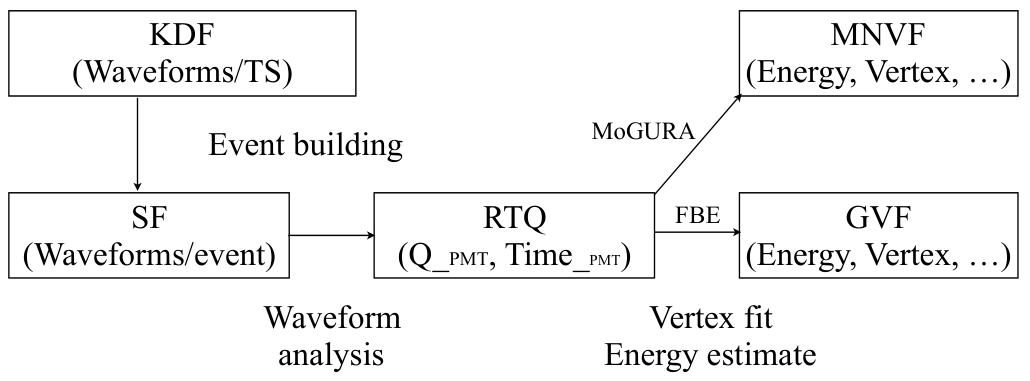
\includegraphics[scale=0.3]{dataflow.png}
	\caption{Data flow in KamLAND from raw waveforms to analysis variables such as energy, vertex, total hit PMTs, etc. \cite{ozaki_phd}}
	\label{fig:dataflow}
\end{figure}

GVF files contain the following information:
\begin{itemize}
	\item \textbf{run number}
	\item \textbf{event number}
	\item \textbf{TimeStamp} based on DAQ clock time (25 nsec for KamFEE, 20 nsec for MoGDAQ)
	\item \textbf{unixtime} is the number of seconds from January 1st in 1970 and used for some run vetos
	\item \textbf{trigger type} records which trigger was used
	\item \textbf{event vertex and badness} event vertices and a radius from detector center is saved, along with a vertex fit quality parameter called badness 
	\item \textbf{energy/energy17} visible energies given by the fitter, energy17 is the energy estimate only using 17-inch PMTs
	\item \textbf{TotalChargeID/17/OD} sum of all PMT charges of each PMT type
	\item \textbf{numhit/numhit17} the number of hit PMTs/17-inch PMTs in each event.
	\item \textbf{NsumMax} a maximum number of hit PMTs in a single DAQ cycle within each event, a "peak" nhit of the event
	\item \textbf{N200OD} Maximum number of simultaneous hit OD pmts within 200nsec windows
	\item \textbf{muon entrance and direction} muon fitter results are recorded.
\end{itemize}

Finally, MoGURA events are associated with muon events acquired in KamFEE DAQ (FBE) and stored in a Muon-Neutron Vector File (MNVF) to search for neutron capture events that occur shortly after muons.

\section{Event Reconstruction}
\subsection{Waveform Analysis}
Each digitized waveform has 128 samples with 1.5ns sample times; this corresponds to a waveform digitization window of 192 ns. The waveforms are processed and TQ reconstructed with the following procedure.
\begin{itemize}
	\item \textbf{Smoothing} Each waveform is smoothed via a running-average first derivate.
	\item \textbf{Baseline adjustment} The baseline of each PMT is collected at the beginning of each run. This baseline is subtracted from each waveform.
	\item \textbf{Peak finding} Peaks are found with running-averaged 1st, 2nd, and 3rd derivatives.
	\item \textbf{Leading-edge and Trailing-edge tag} A leading-edge is stamped as 10ns before the peak voltage. The trailing edge is stamped when the waveform returns to baseline. An example of this time-stamping is shown in Figure \ref{fig:waveform_analysis}
	\item \textbf{Waveform Sum calculation} The waveform is integrated from the leading-edge to the trailing-edge.
\end{itemize}

\begin{figure}[htb]
	\centering
	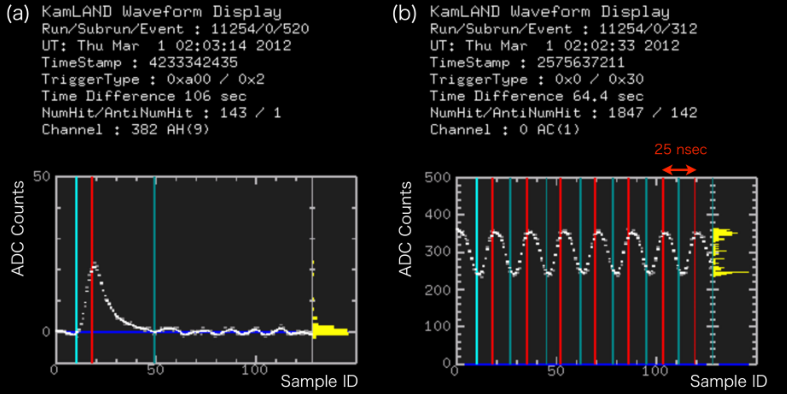
\includegraphics[scale=0.5]{waveform_analysis.png}
	\caption{An example of waveform analysis from thesis \cite{yoshida_phd}. (left) ADC counts of a real waveform after baseline subtraction. The left cyan line is the leading edge, the center red line is the peak position, and the right dark cyan line is a trailing-edge. (right) Clock calibration example on 25 nsec intervals.}
	\label{fig:waveform_analysis}
\end{figure}

When there are mulitple hits in one PMT waveform, the total charge of the hits and the earliest hit time is returned. This simplified information is used for the vertex and energy reconstruction. The multi-pe information is used for a double-pulse fit and a muon shower tag.

\subsection{PMT Corrections}
\subsection*{Low Gain Problem and HV Reductions}
Since ~2011, we observed that the gain of some of the 17-inch PMTs gradually decreased. As the gain of the PMTs fell, this compormises signal/background ratio and PMT waveform quality. It was also observed that the PMTs enter a low impedance state before the gain dropped. A HV current and voltage monitor allows for the real-time monitoring of this state. Usually a simple HV power cycle could recover normal PMT behavior. Since 2016, a auto HV power cycle mechanism was implemented to mitigate the low gain problem, but the root case is still unknown.

Each time the PMTs enter the low impedance state, the HV on that channel was reduced in 50-100 V increments. Over time, some of the channels had their HV reduced by 450 V. FIgure \ref{fig:lowgain_trend} shows the trend in low gain 17-inch PMTs.

\begin{figure}[htb]
	\centering
	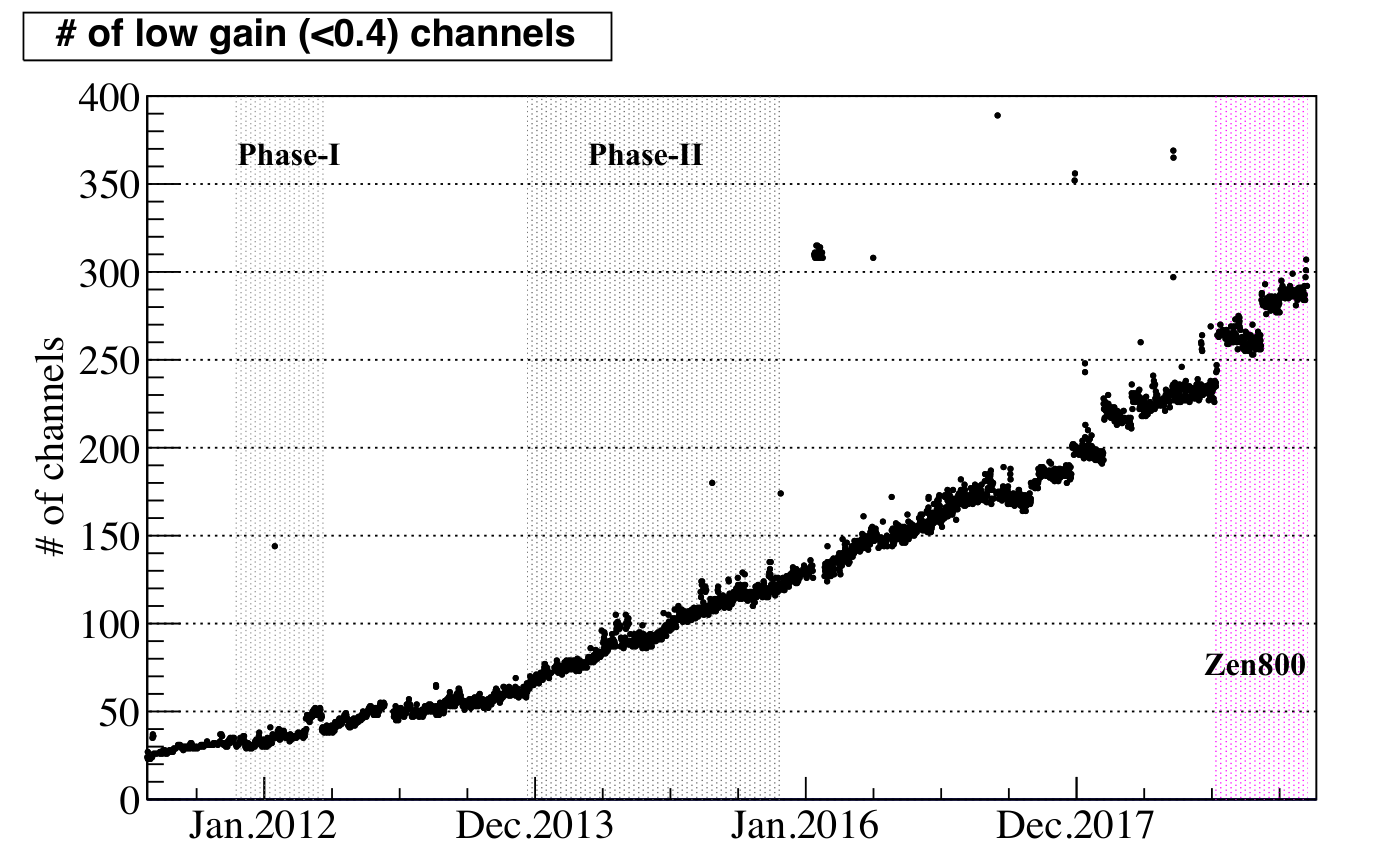
\includegraphics[scale=0.3]{lowgain_trend.png}
	\caption{The trend in the number of low gain 17-inch PMTs, before ZEN-800. The number of low gain channels increased gradually, while the sudden increases are from HV reductions performed since 2017 \cite{ozaki_phd}.}
	\label{fig:lowgain_trend}
\end{figure}

%/ TODO
Note about current low pmt gain analysis.

\subsection*{Bad Channel}
A channels is considered bad if the PMT meets one or more of the following criteria:
\begin{itemize}
	\item PMT pulses less than 0.6\% of the time over all events
	\item PMT pulses below 0.48\% for non-muon events
	\item PMT pulses less than 80\% of the time for high-energy muon events
	\item PMT is missing a waveform more than 10\% of the time
	\item Large discrepancy between the two ATWD hits
	\item High muon charge PMTs. A PMT may read much higher charge ($Q_{detected}$) than the average of its surrounding PMTs ($Q_{expected}$). A run is divided into 100 muon intervals, for each interval the criteria is defined as
	\[\frac{1}{N_{interval}}\sum_{i=1}^{N_{interval}}\left(\frac{1}{N_{muon}}\sum_{j=1}^{N_{muon}}\frac{(Q_{expected}-Q_{detected})^2}{Q_{expected}}\right)>1000\ p.e.\]
\end{itemize}
These bad channels are excluded from event reconstruction and physics analyses.

\subsection*{Dark Hit}
Thermal fluctuations can emit electrons off the photocathode leading to a PMT hit signal. These "dark hits" are an unavoidable hit-level background in PMT detectors, lowering the detector temperature reduces this effect. The dark hit rates are measured from run-to-run and are factored into our likelihood-maximizing reconstruction algorithms. The hit rate observed 50-100 ns before the PMT hittime rising edge is taken as the dark rate, Figure \ref{fig:darkrate} shows the PMT hittime distribution and the dark rate window.

\begin{figure}[htb]
	\centering
	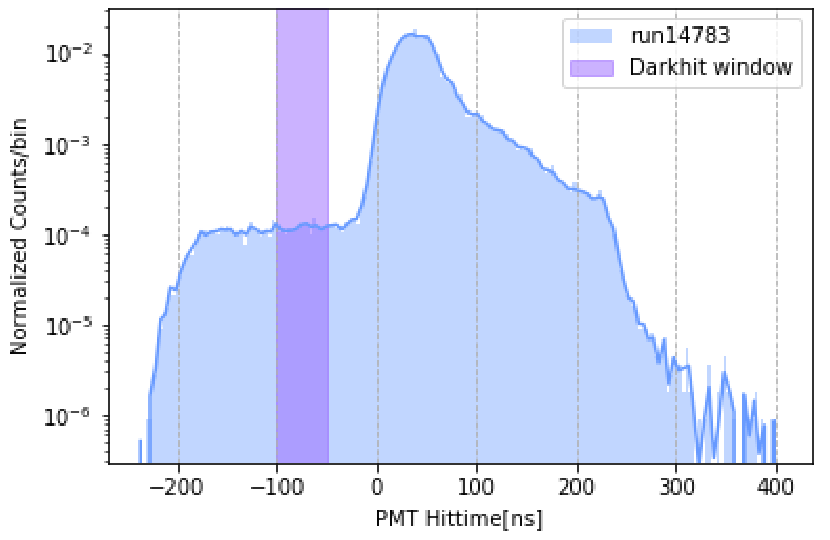
\includegraphics[scale=0.4]{darkrate.png}
	\caption{An example pmt hit time distribution from data run 14783, the 50-100 ns leading window is taken to measure the pmt dark hit rate. \cite{li_phd}.}
	\label{fig:darkrate}
\end{figure}

\subsection{Primary Vertex Fitter}
The primary vertex fitter provides a rough estimate of a scintillating event's location. This estimate serves as the input to a more thorough, but complex secondary fitter. The fit works by constructing a hit time residual distribution:
\begin{equation}
	T_{i}^{emit}=T_i-TOF_i = T_i - \frac{\left|R_i-r_{vertex}\right|}{c_eff}
	\label{eq:prim_vertex}
\end{equation}
Here $T_i$ is the hit time of the $i^{th}$ PMT, $TOF_i$ is the time it takes for a scintillation photon to traverse from the vertex position to the $i^{th}$ PMT position, $R_i$ is the PMT position, $r_{vertex}$ is the unknown vertex position to fit for, and $c_{eff}$ is the speed of light in the given medium. By fitting $T_i^{emit}$ to match the standard scintillation time profile, a primary $r_{vertex}$ is produced by the fitter.

\subsection{Secondary Fitter}
The secondary V2 fitter uses the $r_{vertex}$ given by the primary fitter to compute $T_0$ according to the equation \ref{eq:sec_v2}
\begin{equation}
	T_0 = \frac{\sum_i \left(T_i^{pmt}-TOF^{pmt}_i\right)\times Q_i}{\sum_iQ_i}- const.
	\label{eq:sec_v2}
\end{equation}
\begin{figure}[htb]
	\centering
	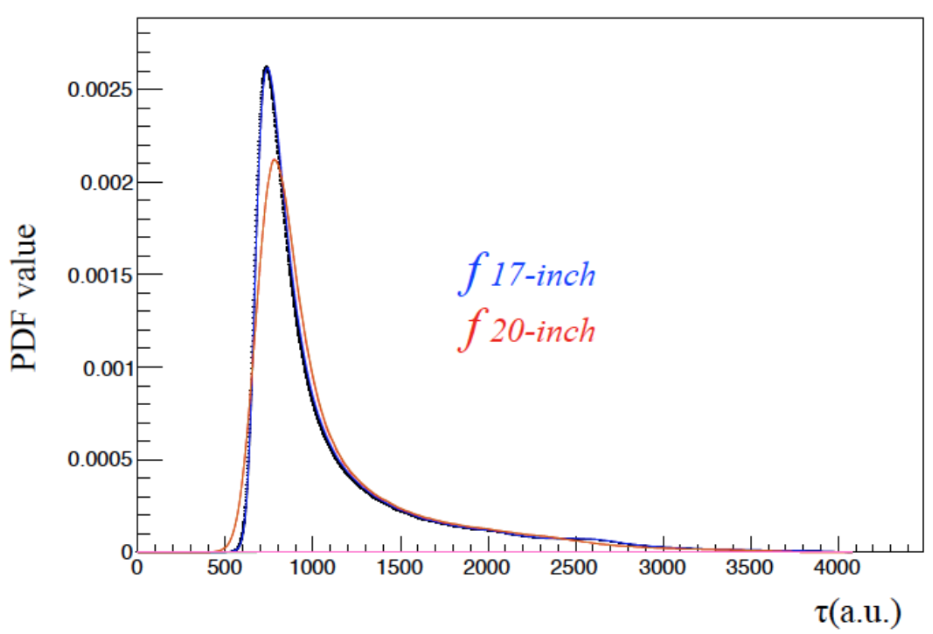
\includegraphics[scale=0.4]{pmt_dist.png}
	\caption{Probability density function of 17-inch and 20-inch PMT hit times calculated from calibration data. The plot is from \cite{ozaki_phd} and originally from a 2005 calibration dataset.}
	\label{fig:pmt_pdfs}
\end{figure}
This $T_0$ is the charge weighted sum of $T_emit$ from \ref{eq:prim_vertex}. This $T_0$ serves as the universal start point of an event. From this time, each pmt hit time is
\begin{equation}
	\tau(x,y,z,T_0) = T^{pomt}_i-TOF_i^{pmt}-T_0
\end{equation}
Finally, these time-of-flight corrected and centered hit time distributions are used to create probability distributions for the 17 and 20 inch PMTs respectively. These PDFs are shown in Figure \ref{fig:pmt_pdfs}. The likelihood function for an individual PMT is defined as:
\begin{equation}
	\phi_i =\frac{\mu\times f_i(\tau_i)+D_i}{\mu\times C_{17/20}+D_i}
\end{equation}
Here, $\mu$ is the pulse shape determination factor, $D_i$ is the dark hit rate for the $i^{th}$ PMT and $C_{17/20}$ is the normalization constant for the 17 or 20 inch PMTs. The overall log-likelihood is given by the $log(L)=\sum_ilog(\phi_i)$. The log-likelihood is maximized by the Newton-Raphson method, in which the $x,y,z,T_0$ are adjusted to the best-fit values, giving us the V2 reconstructed vertex.

\subsection{Energy Reconstruction}
Likelihood maximization is also used to reconstruct the energy of an event. A likelihood PDF is constructed using the number of hits, charge, and hit timing.
\subsection*{$N_{hit}$ PDF}
The expectation of the number of photons hitting PMT i, $\mu_i$ is a function of the visible energy and dark charge.
\begin{equation}
	\mu_i = a_i(x,y,z)\times E_{vis} +d_i
\end{equation}
Here, $a_i(x,y,z)$ is a coefficient that converts the event energy to the number of photons which is calibrated with the neutron events. It is determined by the PMT position $x,y,z$. $d_i$ is the dark noise charge of PMT i, which is electronically measured. The probability that $\mu_i$ photons hit the $i$th PMT $j$ times, $k_{ij}$, is ideally expressed by the poisson distribution:
\begin{equation}
	k_{ij}=\frac{(\mu_i)^j}{j!}e^{-\mu}
\end{equation}

However, in KamLAND waveform analysis, the 1 p.e. detection efficiency is reduced by the 0.3 p.e. software charge threshold. This threshold is set to reduce the acceptance of dark noise but also decreases hit detection efficiency. As a result, the PMT hit probablity is reduced to:
\begin{equation}
	P_{hit}=1-v_ie^{-\mu_i}
\end{equation}

\subsection*{Hit Charge PDF}
A Gaussian distribution is assumed for the hit charge PDF of each PMT:
\begin{equation}
	f_{i,j(q_i)}=\frac{1}{\sqrt{2\pi j\sigma^2}}exp(-\frac{(q_i-j)^2}{2j\sigma^2})
\end{equation}
$q_i$ is the observed charge in p.e. units and $\sigma$ is  the charge resolution against 1 p.e. distribution.

\subsection*{Hit Time PDF}


\subsection{Muon Reconstruction}
\subsection{MoGURA Neutron Reconstruction}
\section{Event Selection}


